\documentclass[12pt]{article}
\usepackage{../preamble3}
%\pagenumbering{gobble}
\title{MathCounts Chapter Invitational February 2021 \\ Sprint Round}
\author{Patrick \& James Toche}
\date{Revised:~\today}

\begin{document}
\maketitle
\begin{minipage}{\textwidth}
\begin{abstract}\setlength{\parindent}{0pt}%
Notes on Sprint Round of MathCounts Invitational Competition, February 2021. 
Questions are from MathCounts Foundation (\url{https://www.mathcounts.org/}). Copyright restrictions may apply. Written for personal use. 
Please report typos and errors over at \url{https://github.com/ptoche/Math/tree/master/mathcounts}. 
\end{abstract}
\end{minipage}

\thispagestyle{empty}
\clearpage
\addtocounter{page}{-1}

\section*{Sprint Round}


%%%%%%%%%%%%%%%%%%%%%%%%%%%%%%%%%%%%%%%%%%%%%%%%%%%%%%%%%%%%%%%%%%%%%%%%
\subsection*{1.}
What is the arithmetic mean of the terms in the arithmetic sequence $12$, $18$, $24$, $30$, $36$?

\nopagebreak

\fbox{\phantom{ANSWER}}

\begin{answer}
\begin{tikzpicture}\node[textbox]{%
    \begin{minipagex}{\dimexpr\textwidth-20pt}
        You could calculate it ($(12+18+24+30+36)/5=24$), but you can get the result without calculations by noting that the mean of an arithmetic sequence is its median, that is if $a$ denotes the increment, we have:
        \begin{center}
        \begin{tabular}{Q{2cm}Q{2cm}Q{2cm}Q{2cm}Q{2cm}}
           12, &   18, & 24, & 30,   & 36 \\
        24-2a, & 24-a, & 24, & 24+a, & 24+2a
        \end{tabular}
        \end{center}
        When you calculate the sum, the $-2a$ term is canceled by $+2a$ and $-a$ is canceled by $+a$, leaving $(5 \times 24)/5=24$.
        \begin{empheq}[box={\mathbox[colback=white]}]{equation*}
            24
        \end{empheq}
    \end{minipagex}
    };
\end{tikzpicture}%
\end{answer}
%%%%%%%%%%%%%%%%%%%%%%%%%%%%%%%%%%%%%%%%%%%%%%%%%%%%%%%%%%%%%%%%%%%%%%%%


%%%%%%%%%%%%%%%%%%%%%%%%%%%%%%%%%%%%%%%%%%%%%%%%%%%%%%%%%%%%%%%%%%%%%%%%
\subsection*{2.}
If Skylar colors $\dfrac{1}{2}$ of $\dfrac{2}{3}$ of the squares in this figure, how many squares does he color?

\begin{minipage}[b]{\linewidth}
  \centering
  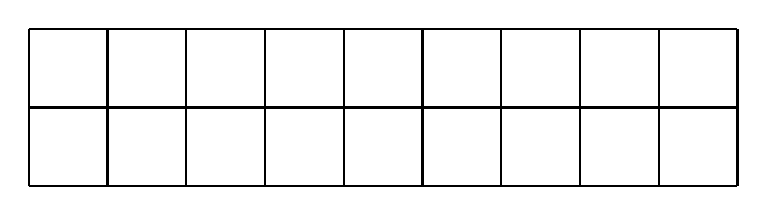
\begin{tikzpicture}
  \foreach \x in {1,...,10}{
    \draw[thick] (\x,0) -- (\x,2) {};
    }
  \foreach \y in {0,...,2}{
    \draw[thick] (1,\y) -- (10,\y) {};
    }
  \end{tikzpicture}
\end{minipage}

\nopagebreak

\fbox{\phantom{ANSWER}}~squares

\begin{answer}
\begin{tikzpicture}\node[textbox]{%
    \begin{minipagex}{\dimexpr\textwidth-20pt}
        There are $9$ columns and $2$ rows. Two-thirds of $9$ columns gives $6$ columns, half of that gives $3$ columns, so $3 \times 2 = 6$.
        \begin{empheq}[box={\mathbox[colback=white]}]{equation*}
            6 ~\text{squares}
        \end{empheq}
    \end{minipagex}
    };
\end{tikzpicture}%
\end{answer}
%%%%%%%%%%%%%%%%%%%%%%%%%%%%%%%%%%%%%%%%%%%%%%%%%%%%%%%%%%%%%%%%%%%%%%%%


%%%%%%%%%%%%%%%%%%%%%%%%%%%%%%%%%%%%%%%%%%%%%%%%%%%%%%%%%%%%%%%%%%%%%%%%
\subsection*{3.}
What is the median of the first seven prime numbers?

\nopagebreak

\fbox{\phantom{ANSWER}}

\begin{answer}
\begin{tikzpicture}\node[textbox]{%
    \begin{minipagex}{\dimexpr\textwidth-20pt}
        The first seven prime numbers are:
        \begin{align*}
        2, 3, 5, 7, 11, 13, 17
        \end{align*}
        so the median is the number in the middle, $7$. 
        \begin{empheq}[box={\mathbox[colback=white]}]{equation*}
            7
        \end{empheq}
    \end{minipagex}
    };
\end{tikzpicture}%
\end{answer}
%%%%%%%%%%%%%%%%%%%%%%%%%%%%%%%%%%%%%%%%%%%%%%%%%%%%%%%%%%%%%%%%%%%%%%%%


%%%%%%%%%%%%%%%%%%%%%%%%%%%%%%%%%%%%%%%%%%%%%%%%%%%%%%%%%%%%%%%%%%%%%%%%
\subsection*{4.}
What is the absolute difference between five less than a number $n$ and seven more than $n$?

\nopagebreak

\fbox{\phantom{ANSWER}}

\begin{answer}
\begin{tikzpicture}\node[textbox]{%
    \begin{minipagex}{\dimexpr\textwidth-20pt}
        The verbal statement may be expressed as
        \begin{align*}
        |(n-5) - (n+7)| = |-12| = 12
        \end{align*}
        \begin{empheq}[box={\mathbox[colback=white]}]{equation*}
            12
        \end{empheq}
    \end{minipagex}
    };
\end{tikzpicture}%
\end{answer}
%%%%%%%%%%%%%%%%%%%%%%%%%%%%%%%%%%%%%%%%%%%%%%%%%%%%%%%%%%%%%%%%%%%%%%%%


%%%%%%%%%%%%%%%%%%%%%%%%%%%%%%%%%%%%%%%%%%%%%%%%%%%%%%%%%%%%%%%%%%%%%%%%
\subsection*{5.}
What is the distance between points $A$ and $B$ on the coordinate grid shown? 

\begin{minipage}[b]{\linewidth}
  \centering
  \includegraphics[height=6cm]{sprint-05-figure}
\end{minipage}

\nopagebreak

\fbox{\phantom{ANSWER}}~units

\begin{answer}
\begin{tikzpicture}\node[textbox]{%
    \begin{minipagex}{\dimexpr\textwidth-20pt}
        The distance between $A$ and $B$ is the hypotenuse of the triangle with side lengths $3$ and $4$. Therefore
        \begin{align*}
        \sqrt{3^2 + 4^2} = 5
        \end{align*}
        This of course is the best-known of the Pythagorean triangles $(3,4,5)$. 
        \begin{empheq}[box={\mathbox[colback=white]}]{equation*}
            5 ~\text{units}
        \end{empheq}
    \end{minipagex}
    };
\end{tikzpicture}%
\end{answer}
%%%%%%%%%%%%%%%%%%%%%%%%%%%%%%%%%%%%%%%%%%%%%%%%%%%%%%%%%%%%%%%%%%%%%%%%


%%%%%%%%%%%%%%%%%%%%%%%%%%%%%%%%%%%%%%%%%%%%%%%%%%%%%%%%%%%%%%%%%%%%%%%%
\subsection*{6.}
Regular hexagon $ABCDEF$, shown here, has area $5$ units$^2$. What is the area of trapezoid $BCDE$? Express your answer as a decimal to the nearest tenth. 

\begin{minipage}[b]{\linewidth}
  \centering
  \includegraphics[height=5cm]{sprint-06-figure}
\end{minipage}

\nopagebreak

\fbox{\phantom{ANSWER}}~units$^2$

\begin{answer}
\begin{tikzpicture}\node[textbox]{%
    \begin{minipagex}{\dimexpr\textwidth-20pt}
        The area of trapezoid $BCDE$ is clearly half of hexagon $ABCDEF$.
        \begin{empheq}[box={\mathbox[colback=white]}]{equation*}
            2.5 ~\text{units}^2
        \end{empheq}
    \end{minipagex}
    };
\end{tikzpicture}%
\end{answer}
%%%%%%%%%%%%%%%%%%%%%%%%%%%%%%%%%%%%%%%%%%%%%%%%%%%%%%%%%%%%%%%%%%%%%%%%


%%%%%%%%%%%%%%%%%%%%%%%%%%%%%%%%%%%%%%%%%%%%%%%%%%%%%%%%%%%%%%%%%%%%%%%%
\subsection*{7.}
What is the value of the expression $\sqrt{9^2-5 \times 4 + 12 \div 4}$

\nopagebreak

\fbox{\phantom{ANSWER}}

\begin{answer}
\begin{tikzpicture}\node[textbox]{%
    \begin{minipagex}{\dimexpr\textwidth-20pt}
        Respecting the order of operations:
        \begin{align*}
        \sqrt{9^2-5 \times 4 + 12 \div 4}
          = \sqrt{81-20 + 3}
          = \sqrt{64}
          = 8
        \end{align*}
        \begin{empheq}[box={\mathbox[colback=white]}]{equation*}
            8
        \end{empheq}
    \end{minipagex}
    };
\end{tikzpicture}%
\end{answer}
%%%%%%%%%%%%%%%%%%%%%%%%%%%%%%%%%%%%%%%%%%%%%%%%%%%%%%%%%%%%%%%%%%%%%%%%


%%%%%%%%%%%%%%%%%%%%%%%%%%%%%%%%%%%%%%%%%%%%%%%%%%%%%%%%%%%%%%%%%%%%%%%%
\subsection*{8.}
Given that $3a+5=7b-11$ and $a=b$, what is the value of $a$?

\nopagebreak

\fbox{\phantom{ANSWER}}

\begin{answer}
\begin{tikzpicture}\node[textbox]{%
    \begin{minipagex}{\dimexpr\textwidth-20pt}
        This simple system of two equations in two unknowns may be solved by substitution:
        \begin{align*}
        3a + 5 & = 7a - 11 \\ 
            4a & = 16 \\
             a & = 4
        \end{align*}
        \begin{empheq}[box={\mathbox[colback=white]}]{equation*}
            4
        \end{empheq}
    \end{minipagex}
    };
\end{tikzpicture}%
\end{answer}
%%%%%%%%%%%%%%%%%%%%%%%%%%%%%%%%%%%%%%%%%%%%%%%%%%%%%%%%%%%%%%%%%%%%%%%%


%%%%%%%%%%%%%%%%%%%%%%%%%%%%%%%%%%%%%%%%%%%%%%%%%%%%%%%%%%%%%%%%%%%%%%%%
\subsection*{9.}
An album with twelve songs costs $\$9.99$. If Andy buys each song individually, he pays $\$0.99$ per song. How much money can Andy save by buying the album instead of each individual song?

\nopagebreak

\fbox{\phantom{ANSWER}}

\begin{answer}
\begin{tikzpicture}\node[textbox]{%
    \begin{minipagex}{\dimexpr\textwidth-20pt}
        Andy can save:
        \begin{align*}
        12 \times 0.99 - 9.99  
          & = (12 \times 1 - 12 \times 0.01) - (10 - 0.01) \\
          & = 2 - 11 \times 0.01 \\
          & = 2 - 0.1 + 0.01 \\
          & = 1.89
        \end{align*}
        \begin{empheq}[box={\mathbox[colback=white]}]{equation*}
            \$~ 1.89
        \end{empheq}
    \end{minipagex}
    };
\end{tikzpicture}%
\end{answer}
%%%%%%%%%%%%%%%%%%%%%%%%%%%%%%%%%%%%%%%%%%%%%%%%%%%%%%%%%%%%%%%%%%%%%%%%


%%%%%%%%%%%%%%%%%%%%%%%%%%%%%%%%%%%%%%%%%%%%%%%%%%%%%%%%%%%%%%%%%%%%%%%%
\subsection*{10.}
What is the integer value of \faPaw ~$\bm{+}$~ \faBirthdayCake ~$\bm{+}$~ \faAutomobile, given these three equations?
\begin{align*}
% The symbols used by MathCounts were:
% \faPaw -> Dog
% \faBirthdayCake -> Ice Cream
% \faAutomobile -> Turtle
\text{\faPaw} ~\bm{+}~ \text{\faPaw} ~\bm{+}~ \text{\faPaw} & \bm{~=~ 90} \\
\text{\faPaw} ~\bm{+}~ \text{\faBirthdayCake} ~\bm{+}~ \text{\faBirthdayCake} & \bm{~=~ 60} \\
\text{\faPaw} ~\bm{+}~ \text{\faPaw} ~\bm{-}~ \text{\faAutomobile} & \bm{~=~ 40}
\end{align*}

\nopagebreak

\fbox{\phantom{ANSWER}}

\begin{answer}
\begin{tikzpicture}\node[textbox]{%
    \begin{minipagex}{\dimexpr\textwidth-20pt}
    \begin{align*}
     \bm{3}~\text{\faPaw} & \bm{~=~ 90 \quad\Rightarrow\quad \text{\faPaw} = 30} \\
     \bm{2}~\text{\faBirthdayCake} & \bm{~=~ 60 -
    \text{\faPaw} \quad\Rightarrow\quad  \text{\faBirthdayCake} = 15} \\
    \text{\faAutomobile} & \bm{~=~ 2~\text{\faPaw} -40 = 20} \\
    \Rightarrow\quad \text{\faPaw} ~\bm{+}~ \text{\faBirthdayCake} ~\bm{+}~ \text{\faAutomobile} & \bm{~=~ 30 + 15 + 20 = 65} 
    \end{align*}
        \begin{empheq}[box={\mathbox[colback=white]}]{equation*}
            65
        \end{empheq}
    \end{minipagex}
    };
\end{tikzpicture}%
\end{answer}
%%%%%%%%%%%%%%%%%%%%%%%%%%%%%%%%%%%%%%%%%%%%%%%%%%%%%%%%%%%%%%%%%%%%%%%%


%%%%%%%%%%%%%%%%%%%%%%%%%%%%%%%%%%%%%%%%%%%%%%%%%%%%%%%%%%%%%%%%%%%%%%%%
\subsection*{11.}
At Alicia's new job, she works three days a week for a total of $45$ hours per week. At her old job, she worked $4$ days a week for a total of $40$ hours per week. What is the absolute difference in the average number of hours Alicia worked per workday at her old and new jobs?

\nopagebreak

\fbox{\phantom{ANSWER}}~hours

\begin{answer}
\begin{tikzpicture}\node[textbox]{%
    \begin{minipagex}{\dimexpr\textwidth-20pt}
        Alicia can save:
        \begin{align*}
        \left|\frac{45}{3} - \frac{40}{4}\right|
          = |15 - 10|
          = 5
        \end{align*}
        \begin{empheq}[box={\mathbox[colback=white]}]{equation*}
            5 ~\text{hours}
        \end{empheq}
    \end{minipagex}
    };
\end{tikzpicture}%
\end{answer}
%%%%%%%%%%%%%%%%%%%%%%%%%%%%%%%%%%%%%%%%%%%%%%%%%%%%%%%%%%%%%%%%%%%%%%%%


%%%%%%%%%%%%%%%%%%%%%%%%%%%%%%%%%%%%%%%%%%%%%%%%%%%%%%%%%%%%%%%%%%%%%%%%
\subsection*{12.}
What is the value of $x$ if $x^x = 256$?

\nopagebreak

\fbox{\phantom{ANSWER}}

\begin{answer}
\begin{tikzpicture}\node[textbox]{%
    \begin{minipagex}{\dimexpr\textwidth-20pt}
        Since $256$ is a power of $2$, so must be $x$. Candidates are then $2$, $4$, $8$, and so on. Thus,
        \begin{align*}
        x^x = 256 \Rightarrow 4^4 = 256 
        \end{align*}
        \begin{empheq}[box={\mathbox[colback=white]}]{equation*}
            4
        \end{empheq}
    \end{minipagex}
    };
\end{tikzpicture}%
\end{answer}
%%%%%%%%%%%%%%%%%%%%%%%%%%%%%%%%%%%%%%%%%%%%%%%%%%%%%%%%%%%%%%%%%%%%%%%%


%%%%%%%%%%%%%%%%%%%%%%%%%%%%%%%%%%%%%%%%%%%%%%%%%%%%%%%%%%%%%%%%%%%%%%%%
\subsection*{13.}
What is the least positive integer that has five distinct prime factors?

\nopagebreak

\fbox{\phantom{ANSWER}}

\begin{answer}
\begin{tikzpicture}\node[textbox]{%
    \begin{minipagex}{\dimexpr\textwidth-20pt}
        Multiply the first five prime numbers:
        \begin{align*}
        2 \times 3 \times 5 \times 7 \times 11 = 3 \times 770 = 2310
        \end{align*}
        \begin{empheq}[box={\mathbox[colback=white]}]{equation*}
            2310
        \end{empheq}
    \end{minipagex}
    };
\end{tikzpicture}%
\end{answer}
%%%%%%%%%%%%%%%%%%%%%%%%%%%%%%%%%%%%%%%%%%%%%%%%%%%%%%%%%%%%%%%%%%%%%%%%


%%%%%%%%%%%%%%%%%%%%%%%%%%%%%%%%%%%%%%%%%%%%%%%%%%%%%%%%%%%%%%%%%%%%%%%%
\subsection*{14.}
Jasmine estimates her maximum heart rate, in beats per minute, by subtracting her age from $220$. Jasmine's heart rate during exercise should be between $50\%$ and $85\%$ of her maximum heart rate. If Jasmine is $20$ years old, what is the highest heart rate, in beats per minute, that she should have during exercise? Express your answer to the nearest whole number. 

\nopagebreak

\fbox{\phantom{ANSWER}}~beats per minute

\begin{answer}
\begin{tikzpicture}\node[textbox]{%
    \begin{minipagex}{\dimexpr\textwidth-20pt}
        The highest rate Jasmine should have, $r_{\text{max}}$, is:
        \begin{align*}
        r_{\text{max}} 
          = 0.85 \times r
          = 0.85 \times (220 - 20)
          = 170	
        \end{align*}
        \begin{empheq}[box={\mathbox[colback=white]}]{equation*}
            170 ~\text{beats per minute}
        \end{empheq}
    \end{minipagex}
    };
\end{tikzpicture}%
\end{answer}
%%%%%%%%%%%%%%%%%%%%%%%%%%%%%%%%%%%%%%%%%%%%%%%%%%%%%%%%%%%%%%%%%%%%%%%%


%%%%%%%%%%%%%%%%%%%%%%%%%%%%%%%%%%%%%%%%%%%%%%%%%%%%%%%%%%%%%%%%%%%%%%%%
\subsection*{15.}
The arithmetic mean of three distinct integers is $11$, and the range of the three integers is $2$. What is the smallest of these integers?

\nopagebreak

\fbox{\phantom{ANSWER}}

\begin{answer}
\begin{tikzpicture}\node[textbox]{%
    \begin{minipagex}{\dimexpr\textwidth-20pt}
        Since the range is $2$, these are three consecutive integers, with the middle integer being $11$, implying that the smallest of the three is $10$. 
        \begin{empheq}[box={\mathbox[colback=white]}]{equation*}
            10
        \end{empheq}
    \end{minipagex}
    };
\end{tikzpicture}%
\end{answer}
%%%%%%%%%%%%%%%%%%%%%%%%%%%%%%%%%%%%%%%%%%%%%%%%%%%%%%%%%%%%%%%%%%%%%%%%


%%%%%%%%%%%%%%%%%%%%%%%%%%%%%%%%%%%%%%%%%%%%%%%%%%%%%%%%%%%%%%%%%%%%%%%%
\subsection*{16.}
Let $a\&b=ab+b+a-1$. If $a\&7=70$, what is $a\&3$?

\nopagebreak

\fbox{\phantom{ANSWER}}~

\begin{answer}
\begin{tikzpicture}\node[textbox]{%
    \begin{minipagex}{\dimexpr\textwidth-20pt}
        A simple matter of substituting $7$ for $b$:
        \begin{align*}
        a\&7 = 70 
        \quad\Rightarrow\quad 
        7a + 7 + a - 1 = 70 
        \quad\Rightarrow\quad 
        a = \frac{70-6}{8} = 8
        \end{align*}
        and then substituting both $8$ for $a$ and $3$ for $b$:
        \begin{align*}
        a\&3 = 8\&3 = 8 \times 3 + 3 + 8 - 1 = 34
        \end{align*}
        \begin{empheq}[box={\mathbox[colback=white]}]{equation*}
            34
        \end{empheq}
    \end{minipagex}
    };
\end{tikzpicture}%
\end{answer}
%%%%%%%%%%%%%%%%%%%%%%%%%%%%%%%%%%%%%%%%%%%%%%%%%%%%%%%%%%%%%%%%%%%%%%%%


%%%%%%%%%%%%%%%%%%%%%%%%%%%%%%%%%%%%%%%%%%%%%%%%%%%%%%%%%%%%%%%%%%%%%%%%
\subsection*{17.}
Kody's alarm rings every $11$ minutes, and his dad calls upstairs every $15$ minutes to wake him up. But Kody will only wake up if his alarm rings and his dad calls him at the same time. If his alarm first rings at $7{:}00$am and his dad first calls him at $7{:}05$a.m., at what time will Kody wake up?

\nopagebreak

\fbox{\phantom{ANSWER}}~a.m.

\begin{answer}
\begin{tikzpicture}\node[textbox]{%
    \begin{minipagex}{\dimexpr\textwidth-20pt}
      \begin{minipage}[b]{\linewidth}
        \centering
        \includegraphics[height=3cm]{sprint-17-figure}
      \end{minipage}                
        \begin{empheq}[box={\mathbox[colback=white]}]{equation*}
            8{:}50 ~\text{a.m.}
        \end{empheq}
    \end{minipagex}
    };
\end{tikzpicture}%
\end{answer}
%%%%%%%%%%%%%%%%%%%%%%%%%%%%%%%%%%%%%%%%%%%%%%%%%%%%%%%%%%%%%%%%%%%%%%%%


%%%%%%%%%%%%%%%%%%%%%%%%%%%%%%%%%%%%%%%%%%%%%%%%%%%%%%%%%%%%%%%%%%%%%%%%
\subsection*{18.}
The largest rectangular region shown is partitioned into three rectangular regions labeled $A$, $B$, and $C$. The lengths, in inches, of rectangles $A$, $B$, and $C$ are $n+3$, $n+5$ and $n-2$, respectively, and all three rectangles have width $n$. If the area of rectangle $B$ is $84$in$^2$, what is the perimeter of the largest rectangle shown?

\begin{minipagex}[b]{\linewidth}
\centering
\includegraphics[height=3cm]{sprint-18-figure}
\end{minipagex}

\nopagebreak

\fbox{\phantom{ANSWER}}~inches

\begin{answer}
\begin{tikzpicture}\node[textbox]{%
    \begin{minipagex}{\dimexpr\textwidth-20pt}
        The area of rectangle $B$ is $n(n+5)$, which yields a quadratic equation in $n$:
        \begin{align*}
           n^2 + 5n = 84
        \end{align*}
        Completing the square:
        \begin{align*}
           n^2 + 5n & = 84 \\
           \left(n + \frac{5}{2}\right)^2 - \left(\frac{5}{2}\right)^2 & = 84 \\
           \left(n + \frac{5}{2}\right)^2 - \left(\frac{25+4 \times 84}{2^2}\right) & = 0 \\
           \left(n + \frac{5}{2}\right)^2 - \left(\frac{19}{2}\right)^2 & = 0 
        \end{align*}
        where the last step follows from $25+4\times84=25+336=361=19^2$.
        To complete the square, recall that $a^2-b^2=(a-b)(a+b)$. Thus,
        \begin{align*}
           \left(n+\frac{5}{2}\right)^2-\left(\frac{19}{2}\right)^2 & = 0 \\
           \left(n+\frac{5}{2}-\frac{19}{2}\right)  \left(n+\frac{5}{2}+\frac{19}{2}\right) & = 0 \\
\left(n+\frac{5}{2}+\frac{19}{2}\right) & = 0 
        \end{align*}
        Since $n$ must be positive, we have
        \begin{align*}
           n = -\frac{5}{2}+\frac{19}{2}
             = \frac{14}{2}
             7
        \end{align*}         
        The perimeter of the largest rectangle is 
        \begin{align*}
        2 \times [n + (n+3) + (n+5) + (n-2)] 
          = 2 (3n+6) 
          = 6(n+2)
          = 6...
        \end{align*}
        \begin{empheq}[box={\mathbox[colback=white]}]{equation*}
            68 ~\text{inches}
        \end{empheq}
    \end{minipagex}
    };
\end{tikzpicture}%
\end{answer}
%%%%%%%%%%%%%%%%%%%%%%%%%%%%%%%%%%%%%%%%%%%%%%%%%%%%%%%%%%%%%%%%%%%%%%%%


%%%%%%%%%%%%%%%%%%%%%%%%%%%%%%%%%%%%%%%%%%%%%%%%%%%%%%%%%%%%%%%%%%%%%%%%
\subsection*{19.}
What is the length of the longest diagonal of the rectangular prism shown, which has length $9$\,cm, width $8$\,cm and height $12$\,cm?

\begin{minipagex}[b]{\linewidth}
\centering
\includegraphics[height=5cm]{sprint-19-figure}
\end{minipagex}

\nopagebreak

\fbox{\phantom{ANSWER}}~cm

\begin{answer}
\begin{tikzpicture}\node[textbox]{%
    \begin{minipagex}{\dimexpr\textwidth-20pt}
        \begin{empheq}[box={\mathbox[colback=white]}]{equation*}
            17 ~\text{cm}
        \end{empheq}
    \end{minipagex}
    };
\end{tikzpicture}%
\end{answer}
%%%%%%%%%%%%%%%%%%%%%%%%%%%%%%%%%%%%%%%%%%%%%%%%%%%%%%%%%%%%%%%%%%%%%%%%


%%%%%%%%%%%%%%%%%%%%%%%%%%%%%%%%%%%%%%%%%%%%%%%%%%%%%%%%%%%%%%%%%%%%%%%%
\subsection*{20.}
Suppose there is an $80\%$ chance of rain each day. On days that it rains, Kathy has a $45\%$ chance of being late, compared to a $30\%$ chance when it does not rain. On a random day, what is the probability that Kathy will be late?

\nopagebreak

\fbox{\phantom{ANSWER}}~\%

\begin{answer}
\begin{tikzpicture}\node[textbox]{%
    \begin{minipagex}{\dimexpr\textwidth-20pt}
        A
        \begin{align*}
        0
        \end{align*}
        \begin{empheq}[box={\mathbox[colback=white]}]{equation*}
            42 \%
        \end{empheq}
    \end{minipagex}
    };
\end{tikzpicture}%
\end{answer}
%%%%%%%%%%%%%%%%%%%%%%%%%%%%%%%%%%%%%%%%%%%%%%%%%%%%%%%%%%%%%%%%%%%%%%%%


%%%%%%%%%%%%%%%%%%%%%%%%%%%%%%%%%%%%%%%%%%%%%%%%%%%%%%%%%%%%%%%%%%%%%%%%
\subsection*{21.}
Triangle $ABC$ has sides of length $11$ inches, $15$ inches and $16$ inches. What is the length of the altitude to the side of length $15$ inches? Express your answer in simplest radical form. 

\nopagebreak

\fbox{\phantom{ANSWER}}$\sqrt{\fbox{\phantom{ANSWER}}}$

\begin{answer}
\begin{tikzpicture}\node[textbox]{%
    \begin{minipagex}{\dimexpr\textwidth-20pt}
        A
        \begin{align*}
        0
        \end{align*}
        \begin{empheq}[box={\mathbox[colback=white]}]{equation*}
            4\sqrt{7}
        \end{empheq}
    \end{minipagex}
    };
\end{tikzpicture}%
\end{answer}
%%%%%%%%%%%%%%%%%%%%%%%%%%%%%%%%%%%%%%%%%%%%%%%%%%%%%%%%%%%%%%%%%%%%%%%%


%%%%%%%%%%%%%%%%%%%%%%%%%%%%%%%%%%%%%%%%%%%%%%%%%%%%%%%%%%%%%%%%%%%%%%%%
\subsection*{22.}
Julie is packing marbles into boxes. She needs to pack away $815$ marbles. She has boxes that can hold $10$, $25$, $50$ or $100$ marbles. If Julie can use at most $5$ boxes of each size and must fill each box she uses, what is the minimum number of boxes she needs to pack all her marbles?

\nopagebreak

\fbox{\phantom{ANSWER}}~boxes

\begin{answer}
\begin{tikzpicture}\node[textbox]{%
    \begin{minipagex}{\dimexpr\textwidth-20pt}
        A
        \begin{align*}
        0
        \end{align*}
        \begin{empheq}[box={\mathbox[colback=white]}]{equation*}
            15 ~\text{boxes}
        \end{empheq}
    \end{minipagex}
    };
\end{tikzpicture}%
\end{answer}
%%%%%%%%%%%%%%%%%%%%%%%%%%%%%%%%%%%%%%%%%%%%%%%%%%%%%%%%%%%%%%%%%%%%%%%%


%%%%%%%%%%%%%%%%%%%%%%%%%%%%%%%%%%%%%%%%%%%%%%%%%%%%%%%%%%%%%%%%%%%%%%%%
\subsection*{23.}
What positive number $x$ has the property that $\sqrt[6]{x^7}-6\sqrt[3]{x^2}=0$?

\nopagebreak

\fbox{\phantom{ANSWER}}

\begin{answer}
\begin{tikzpicture}\node[textbox]{%
    \begin{minipagex}{\dimexpr\textwidth-20pt}
        \begin{empheq}[box={\mathbox[colback=white]}]{equation*}
            36
        \end{empheq}
    \end{minipagex}
    };
\end{tikzpicture}%
\end{answer}
%%%%%%%%%%%%%%%%%%%%%%%%%%%%%%%%%%%%%%%%%%%%%%%%%%%%%%%%%%%%%%%%%%%%%%%%


%%%%%%%%%%%%%%%%%%%%%%%%%%%%%%%%%%%%%%%%%%%%%%%%%%%%%%%%%%%%%%%%%%%%%%%%
\subsection*{24.}
What fraction is equivalent to $0.7\overline{12}$? Express your answer as a common fraction. 

\nopagebreak

\begin{minipage}[b]{\linewidth}
\fbox{\phantom{ANSWER}}\\
\mbox{---------------}\\
\fbox{\phantom{ANSWER}}
\end{minipage}


\begin{answer}
\begin{tikzpicture}\node[textbox]{%
    \begin{minipagex}{\dimexpr\textwidth-20pt}
        \begin{empheq}[box={\mathbox[colback=white]}]{equation*}
            \frac{47}{66}
        \end{empheq}
    \end{minipagex}
    };
\end{tikzpicture}%
\end{answer}
%%%%%%%%%%%%%%%%%%%%%%%%%%%%%%%%%%%%%%%%%%%%%%%%%%%%%%%%%%%%%%%%%%%%%%%%


%%%%%%%%%%%%%%%%%%%%%%%%%%%%%%%%%%%%%%%%%%%%%%%%%%%%%%%%%%%%%%%%%%%%%%%%
\subsection*{25.}
In the figure, two circles of radius $1$ inch are internally tangent to a circle of radius $5$ inches so that the centers of all tree circles are collinear. The shaded fourth circle is tangent to each of the other three circles as shown. What is the radius of the shaded circle? Express your answer as a common fraction. 

\begin{minipagex}[b]{\linewidth}
\centering
\includegraphics[height=7cm]{sprint-25-figure}
\end{minipagex}

\nopagebreak

\begin{minipage}[b]{\linewidth}
\fbox{\phantom{ANSWER}}\\
\mbox{---------------}\\
\fbox{\phantom{ANSWER}}
\end{minipage}

\begin{answer}
\begin{tikzpicture}\node[textbox]{%
    \begin{minipagex}{\dimexpr\textwidth-20pt}
        \begin{empheq}[box={\mathbox[colback=white]}]{equation*}
            \frac{10}{3}
        \end{empheq}
    \end{minipagex}
    };
\end{tikzpicture}%
\end{answer}
%%%%%%%%%%%%%%%%%%%%%%%%%%%%%%%%%%%%%%%%%%%%%%%%%%%%%%%%%%%%%%%%%%%%%%%%


%%%%%%%%%%%%%%%%%%%%%%%%%%%%%%%%%%%%%%%%%%%%%%%%%%%%%%%%%%%%%%%%%%%%%%%%
\subsection*{26.}
The greatest of three nonnegative integers is one more than twice the sum of the other two integers. The arithmetic mean of the three integers, rounded to the nearest integer, happens to equal the median of the set. What is the product of the three integers?

\nopagebreak

\fbox{\phantom{ANSWER}}

\begin{answer}
\begin{tikzpicture}\node[textbox]{%
    \begin{minipagex}{\dimexpr\textwidth-20pt}
        \begin{empheq}[box={\mathbox[colback=white]}]{equation*}
            0
        \end{empheq}
    \end{minipagex}
    };
\end{tikzpicture}%
\end{answer}
%%%%%%%%%%%%%%%%%%%%%%%%%%%%%%%%%%%%%%%%%%%%%%%%%%%%%%%%%%%%%%%%%%%%%%%%


%%%%%%%%%%%%%%%%%%%%%%%%%%%%%%%%%%%%%%%%%%%%%%%%%%%%%%%%%%%%%%%%%%%%%%%%
\subsection*{27.}
Suppose $p(x)$ is a polynomial such that $p(x) = p(1) + p(2) \cdot x + x^2$ for all numbers $x$. What is the value of $p(5)$?

\nopagebreak

\fbox{\phantom{ANSWER}}

\begin{answer}
\begin{tikzpicture}\node[textbox]{%
    \begin{minipagex}{\dimexpr\textwidth-20pt}
        A
        \begin{align*}
        0
        \end{align*}
        \begin{empheq}[box={\mathbox[colback=white]}]{equation*}
            x ~\text{y}
        \end{empheq}
    \end{minipagex}
    };
\end{tikzpicture}%
\end{answer}
%%%%%%%%%%%%%%%%%%%%%%%%%%%%%%%%%%%%%%%%%%%%%%%%%%%%%%%%%%%%%%%%%%%%%%%%


%%%%%%%%%%%%%%%%%%%%%%%%%%%%%%%%%%%%%%%%%%%%%%%%%%%%%%%%%%%%%%%%%%%%%%%%
\subsection*{28.}
Let $FLOOR n$ be defined as the greatest integer less than or equal to $n$. What is the value of $n$ if $FLOOR n \times n = 3$? Express your answer as a decimal to the nearest tenth. 

\nopagebreak

\fbox{\phantom{ANSWER}}

\begin{answer}
\begin{tikzpicture}\node[textbox]{%
    \begin{minipagex}{\dimexpr\textwidth-20pt}
        \begin{empheq}[box={\mathbox[colback=white]}]{equation*}
            -1.5
        \end{empheq}
    \end{minipagex}
    };
\end{tikzpicture}%
\end{answer}
%%%%%%%%%%%%%%%%%%%%%%%%%%%%%%%%%%%%%%%%%%%%%%%%%%%%%%%%%%%%%%%%%%%%%%%%


%%%%%%%%%%%%%%%%%%%%%%%%%%%%%%%%%%%%%%%%%%%%%%%%%%%%%%%%%%%%%%%%%%%%%%%%
\subsection*{29.}
Square $ABCD$, shown here, has side length $6$ units. Points $P$ and $Q$ are located on sides $AD$ and $BC$, respectively, with $AP=BQ=1$ unit. Triangles $ACP$ and $BDQ$ overlap in the square to form the shaded quadrilateral. What is the area of the shaded quadrilateral? Express your answer as a common fraction. 

\begin{minipagex}[b]{\linewidth}
\centering
\includegraphics[height=3cm]{sprint-29-figure}
\end{minipagex}

\nopagebreak

\begin{minipage}[b]{\linewidth}
\fbox{\phantom{ANSWER}}\\
\mbox{---------------}~~units$^2$\\
\fbox{\phantom{ANSWER}}
\end{minipage}


\begin{answer}
\begin{tikzpicture}\node[textbox]{%
    \begin{minipagex}{\dimexpr\textwidth-20pt}
        \begin{empheq}[box={\mathbox[colback=white]}]{equation*}
            \frac{3}{22}~\text{units}^2
        \end{empheq}
    \end{minipagex}
    };
\end{tikzpicture}%
\end{answer}
%%%%%%%%%%%%%%%%%%%%%%%%%%%%%%%%%%%%%%%%%%%%%%%%%%%%%%%%%%%%%%%%%%%%%%%%


%%%%%%%%%%%%%%%%%%%%%%%%%%%%%%%%%%%%%%%%%%%%%%%%%%%%%%%%%%%%%%%%%%%%%%%%
\subsection*{30.}
How many ordered triples of positive integers $(a,b,c)$ have $GCF(a,b,c)=2020$ and $LCM(a,b,c)=2020^2$?

\nopagebreak

\fbox{\phantom{ANSWER}}~ordered triples

\begin{answer}
\begin{tikzpicture}\node[textbox]{%
    \begin{minipagex}{\dimexpr\textwidth-20pt}
        \begin{align*}
        XXXX
        \end{align*}
        They each have to be $5^1$ or $5^2$.
        So the powers of $5$ can be $5^1$, $5^1$, $5^2$ or $5^1$, $5^2$, $5^2$. IN how many ways can we assign each of those to $a$, $b$, and $c$? We can assign each pattern to $a$, $b$, $c$ in $3$ different ways, that is: choose whichever of the exponents is different from the other two. This gives $6$ ways to assign the powers of $5$. How about the powers of $101$? Likewise, there are $6$ ways to assign the powers of $101$. The total number of ways is obtained by multiplying the three cases, since the choice of the exponents for each prime are independent of each other:  
        \begin{align*}
        12 \times 6 \times 6 = 432
        \end{align*}
        \begin{empheq}[box={\mathbox[colback=white]}]{equation*}
            432 ~\text{ordered triples}
        \end{empheq}
    \end{minipagex}
    };
\end{tikzpicture}%
\end{answer}
%%%%%%%%%%%%%%%%%%%%%%%%%%%%%%%%%%%%%%%%%%%%%%%%%%%%%%%%%%%%%%%%%%%%%%%%


\end{document}